\documentclass[a7paper,print]{kartei}
\usetikzlibrary{positioning,calc}

\usepackage[utf8]{inputenc}

\begin{document}

\begin{karte}[CGIS]{Was ist das Kreuzprodukt zweier Vektoren im 3-dimensionalen und wie berechnet man es?}
Das Kreuzprodukt ergibt einen Vektor, der senkrecht auf der aufgespannten Fläche der beiden Operanden steht. Der Betrag des neuen Vektors entspricht dem Flächeninhalt der aufgespannten Fläche.\\
Berechnet wird es durch die folgende Formel:\\
$ \overrightarrow{a} \times \overrightarrow{b} = \left( \begin{array}{c} a_1 \\ a_2 \\ a_3 \end{array} \right) \times \left( \begin{array}{c} b_1 \\ b_2 \\ b_3 \end{array} \right)
=
\left(
   \begin{array}{c}
     a_2b_3 - a_3b_2 \\
     a_3b_1 - a_1b_3 \\
     a_1b_2 - a_2b_1
   \end{array}
\right)$
\end{karte}

\begin{karte}[CGIS]{Was ist Auslöschung?}
Genauigkeitsverlust bei Rechenoperationen in IEEE754, tritt auf, falls eine Rechenoperation den relativen Fehler viel mehr als den absoluten erhöht. Die Subtraktion zweier ähnlicher und großer Zahlen endet in Auslöschung.
\end{karte}

\begin{karte}[CGIS]{Verschiebungsmatrix um t}[Transformationen]
$ T(t) = T(t_x,t_y,t_z) = \left( \begin{array}{cccc}
1 & 0 & 0 & t_x \\
0 & 1 & 0 & t_y \\
0 & 0 & 1 & t_z \\
0 & 0 & 0 & 1 \\
\end{array}
\right)
$
\end{karte}

\begin{karte}[CGIS]{Rotationsmatrix um die x-Achse um $\Theta$}[Transformationen]
$ R_x(\Theta) = \left( \begin{array}{cccc}
1 & 0 & 0 & 0 \\
0 & \cos \Theta & -\sin\Theta & 0 \\
0 & \sin \Theta & \cos \Theta & 0 \\
0 & 0 & 0 & 1 \\
\end{array}
\right)
$
\end{karte}

\begin{karte}[CGIS]{Rotationsmatrix um die y-Achse um $\Theta$}[Transformationen]
$ R_y(\Theta) = \left( \begin{array}{cccc}
\cos \Theta & 0 & \sin \Theta & 0 \\
0 & 1 & 0 & 0 \\
-\sin\Theta & 0 & \cos \Theta & 0 \\
0 & 0 & 0 & 1 \\
\end{array}
\right)
$
\end{karte}

\begin{karte}[CGIS]{Rotationsamtrix um die z-Achse um $\Theta$}[Transformationen]
$ R_z(\Theta) = \left( \begin{array}{cccc}
\cos\Theta & -\sin\Theta & 0 & 0 \\
\sin\Theta & \cos\Theta & 0 & 0 \\
0 & 0 & 1 & 0 \\
0 & 0 & 0 & 1 \\
\end{array}
\right)
$
\end{karte}

\begin{karte}[CGIS]{Rotation um einen Punkt $P$ in Abhängigkeit der Verschiebungsmatrix um t und $\Theta$}[Transformationen]
$T(P) R_{\{x,y,z\}}(\Theta) T(-P)$
\end{karte}

\begin{karte}[CGIS]{Scherungsmatrix, geschert um $s$}[Transformationen]
$ H(s) = \left( \begin{array}{cccc}
1 & s_{xy} & s_{xz} & 0 \\
s_{yx} & 1 & s_{yz} & 0 \\
s_{zx} & s_{zy} & 1 & 0 \\
0 & 0 & 0 & 1 \\
\end{array}
\right)
$
\end{karte}

\begin{karte}[CGIS]{Mit welcher Formel kann man den Schnittpunkt der Linie $L(t)=P_0 + t \cdot \overrightarrow{d}$ mit der Polygonkante $\overrightarrow{E_n E_{n+1}}$?}[Transformationen]
$S_i = P_0 + \frac{(E_n - P_0) \overrightarrow{n}}{\overrightarrow{d} \cdot \overrightarrow{n}} \cdot \overrightarrow{d}$
\end{karte}

\begin{karte}[CGIS]{Farbberechnung des Punktes P in folgendem Dreieck: 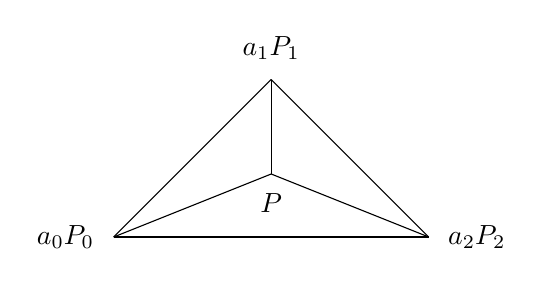
\begin{tikzpicture}
\node[label={left:$a_0P_0$}] (0) at (0,0) {};
\node[label={above:$a_1P_1$}] (1) at (2,2) {};
\node[label={right:$a_2P_2$}] (2) at (4,0) {};
\node[label={below:$P$}] (p) at (2,0.8) {};
\draw[-](0.center)--(1.center);
\draw[-](1.center)--(2.center);
\draw[-](0.center)--(2.center);
\draw[-](0.center)--(p.center);
\draw[-](1.center)--(p.center);
\draw[-](2.center)--(p.center);
\end{tikzpicture}}[Baryzentr. Koordinaten]
\noindent $a_x =$ Farbe (Masse) des Punktes \\
$P_x =$ baryzentrische Koordinaten des Punktes \\
$t_x =$ normierte baryzentrische Koordinate $= \frac{P_x}{P_1+P_2+P_3}\\
a_p = a_o \cdot t_0 + a_1 cdot t_1 + a_2 \cdot t_2 \leftarrow$ Farbe
\end{karte}

\begin{karte}[CGIS]{Farbberechnung des Punktes P in folgendem Dreieck: Berechnung über die Fläche der entstehenden Teildreiecke}[Baryzentr. Koordinaten]
\noindent Das ganze Dreieck hat den Flächeninhalt $F$, wobei gilt:
\begin{itemize}
\item $F=F_{P_0} + F_{P_1} + F_{P_2}$
\item $F_{P_0} = F(\Delta P_0P_1P)$, \\$F_{P_1} = F(\Delta P_1P_2P)$, \\$F_{P_2} = F(\Delta P_2P_0P)$
\item baryzentrische Koordinaten von P haben die Form $(a,b,c)$, wobei gilt: $a=\frac{F_{P_0}}{F}$, $b=\frac{F_{P_1}}{F}$, $c=\frac{F_{P_2}}{F}$
\end{itemize}
\end{karte}

\begin{karte}[CGIS]{Berechnung der Fläche eines Dreieckes über die Vektoren $v_0=P_1-P_0$, $v_1=P_2-P_0$}[Baryzentr. Koordinaten]
$F=\frac{1}{2} \parallel v_0 \times v_1 \parallel = \frac{1}{2} \parallel (P_1-P_0) \times (P_2 - P_0) \parallel \\
= \frac{1}{2} \left| \begin{array}{ccc}
A_x & B_x & C_x \\
A_y & B_y & C_y \\
1 & 1& 1
\end{array}
\right|\\
 = \frac{1}{2} (A_xB_y + B_xC_y + C_x+A_y - A_xC_y - B_xA_y - C_xB_y)$
\end{karte}

\begin{karte}[CGIS]{Abbildung mittels Projektionsmatrix auf kanonisches Volumen $[-1,1]^3$ (Pyramidenstumpf) (Perspektivische Projektionsmatrix)}[Transformationen]
$M_{per} = \left( \begin{array}{cccc}
\frac{2n}{r-l} & 0 & \frac{r+l}{r-l} & 0 \\
0 & \frac{2n}{t-b} & \frac{t+b}{t-b} & 0 \\
0 & 0 & \frac{n+f}{n-f} & \frac{2fn}{n-f}\\
0 & 0 & -1 & 1
\end{array}
\right)$
\end{karte}

\begin{karte}[CGIS]{orthografische Projektionsmatrix des Projektionswürfels $[l;r] \times [b;t]\times [f;n]$}[Transformationen]
$M_{ortho} = S(s)T(t) \\\\
= \left( \begin{array}{cccc}
\frac{2}{r-l} & 0 & 0 & -\frac{l+r}{l-r} \\
0 & \frac{2}{t-b} & 0 & -\frac{t+b}{t-b} \\
0 & 0 & \frac{2}{f-n} & -\frac{f+n}{f-n}\\
0 & 0 & 0 & 1
\end{array}
\right)$
\end{karte}

\begin{karte}[CGIS]{perspektivische Projektionsmatrix (mit Berechnung der Projektions- und orthografischen Matrix)}[Transformationen]
$M_{ortho}^{-1} \cdot M_{per} \\\\
= \left( \begin{array}{cccc}
\frac{r-l}{2} & 0 & 0 & \frac{r+l}{2} \\
0 & \frac{t-b}{2} & 0 & \frac{t+b}{2} \\
0 & 0 & \frac{f-n}{2} & \frac{f+n}{2}\\
0 & 0 & 0 & 1
\end{array}
\right) \cdot 
\left( \begin{array}{cccc}
\frac{2n}{r-l} & 0 & \frac{r+l}{r-l} & 0 \\
0 & \frac{2n}{t-b} & \frac{t+b}{t-b} & 0 \\
0 & 0 & \frac{n+f}{n-f} & \frac{2fn}{n-f}\\
0 & 0 & -1 & 1
\end{array}
\right)\\
= \left( \begin{array}{cccc}
n & 0 & 0 & \frac{r+l}{2} \\
0 & n & 0 & \frac{t+b}{2} \\
0 & 0 & -1 & \frac{f+n}{2}-fn\\
0 & 0 & -1 & 1
\end{array}
\right)$
\end{karte}

\begin{karte}[CGIS]{Visualisierung}[Graph. Datenverarb.]
\noindent Messdaten $\rightarrow$ Bild \\
Daten $\leftrightarrow$ Bild
\end{karte}

\begin{karte}[CGIS]{Lichtsimulation in der Computergrafik\\ \ \\
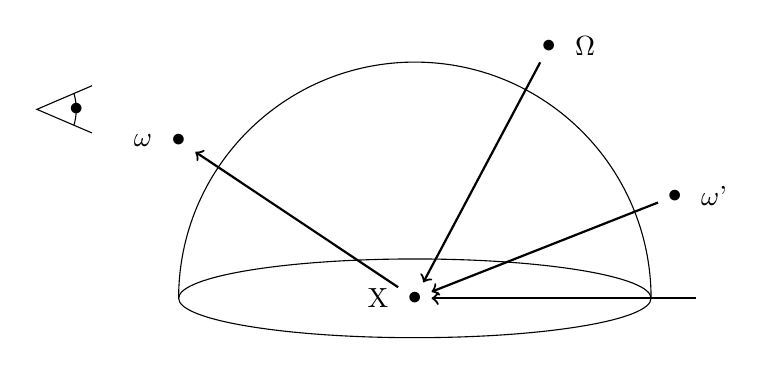
\begin{tikzpicture}[node distance=1cm]
\node[label={left:X}] (0) at (0,0) {$\bullet$};
\draw (0,0) ellipse (3 and .5);
\draw (0:3cm) arc (0:180:3cm);
\node[label={left:$\omega$}](1) at (-3,2){$\bullet$};
\node[label={right:$\omega$'}](2) at (3.3,1.3){$\bullet$};
\node[label={right:$\Omega$}](3) at (1.7,3.2){$\bullet$};
\node(4) at (3.7,0){};
\node(eye) at (-4.8,2.4){};
\node(eye1) at (-4.1,2.7){};
\node(eye2) at (-4.1,2.1){};
\draw[name=1] (eye1.center)--(eye.center)--(eye2.center);
\node(eye3) at (-4.3,2.4){$\bullet$};
\draw [xshift=-4.8cm, yshift=2.4cm](0:.5cm) arc (0:-17:.7cm);
\draw [xshift=-4.8cm, yshift=2.4cm](0:.5cm) arc (0:17:.7cm);
\draw[->,thick] (0)--(1);
\draw[->,thick] (3)--(0);
\draw[->,thick] (2)--(0);
\draw[->,thick] (4)--(0);
\end{tikzpicture}
}[Graph. Datenverarb.]
$L(X,\omega) = L_e(X,\omega)+\int f_r(X, \omega',\omega) L_i (X,\omega')(-\omega' \cdot n) dw$
\end{karte}

\begin{karte}[CGIS]{Auf welche Arten können Objekte beschrieben werden?}[Fragmentbearbeitung]
\begin{itemize}
\item Vertices
\item Gitternetz
\item Oberfläche
\end{itemize}
\end{karte}

\begin{karte}[CGIS]{Aufbau}[Grafik-Pipeline]
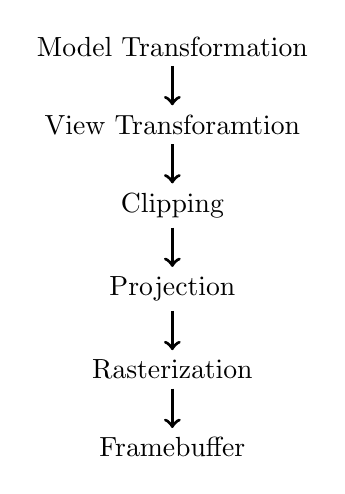
\begin{tikzpicture}[node distance=.5cm]
\node (0) at (0,0) {Model Transformation};
\node (1) [below=of 0] {View Transforamtion};
\node (2) [below=of 1] {Clipping};
\node (3) [below=of 2] {Projection};
\node (4) [below=of 3] {Rasterization};
\node (5) [below=of 4] {Framebuffer};
\draw[->,very thick](0)--(1);
\draw[->,very thick](1)--(2);
\draw[->,very thick](2)--(3);
\draw[->,very thick](3)--(4);
\draw[->,very thick](4)--(5);
\end{tikzpicture}
\end{karte}

\begin{karte}[CGIS]{Vor- und Nachteile}[Grafik-Pipeline]
\begin{itemize}
\item Vorteile:
	\begin{enumerate}
	\item unabhängige Verarbeitung
	\item parallele Ausführung
	\item hohe Geschwindigkeit
	\end{enumerate}
\item Nachteile:
	\begin{enumerate}
	\item keine Beziehung zwischen Objekten
	\item keine Volumeninformationen
	\item Einschränkung durch spezielle Betrachtungsweise
	\end{enumerate}
\end{itemize}
\end{karte}

\begin{karte}[CGIS]{Model Transforamtion: Input}[Grafik-Pipeline]
\begin{itemize}
\item Objektbeschreibungen (Vertices...)
\item Kameraposition
\item Viewport (Fenstergröße)
\item Beleuchtungsmodell
\end{itemize}
\end{karte}

\begin{karte}[CGIS]{Weg der Daten zum Bildschirm (ohne Grafik-Pipeline)}[Graph. Datenverarb.]
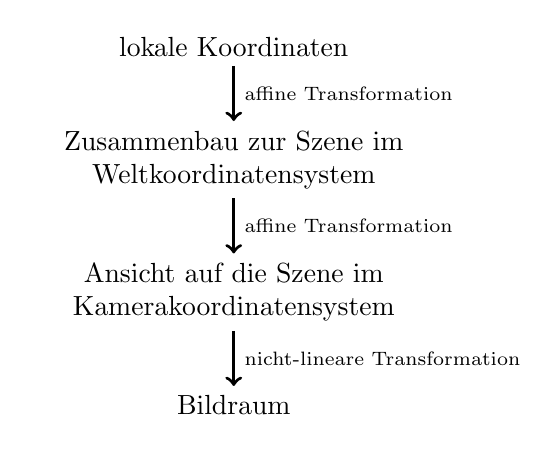
\begin{tikzpicture}[node distance=0.7cm]
\node (0) at (0,0) {\begin{minipage}{5cm}\centering lokale Koordinaten \end{minipage}};
\node (1) [below=of 0] {\begin{minipage}{5cm}\centering Zusammenbau zur Szene im Weltkoordinatensystem\end{minipage}};
\node (2) [below=of 1] {\begin{minipage}{5cm}\centering Ansicht auf die Szene im Kamerakoordinatensystem \end{minipage}};
\node (3) [below=of 2] {\begin{minipage}{5cm}\centering Bildraum \end{minipage}};
\draw[->,very thick](0)to node[right] {\scriptsize{affine Transformation}}(1);
\draw[->,very thick](1)tonode[right] {\scriptsize{affine Transformation}}(2);
\draw[->,very thick](2)tonode[right] {\scriptsize{nicht-lineare Transformation}}(3);
\end{tikzpicture}
\end{karte}

\begin{karte}[CGIS]{Weg der Daten zum Bildschirm (mit Grafik-Pipeline)}[Graph. Datenverarb.]
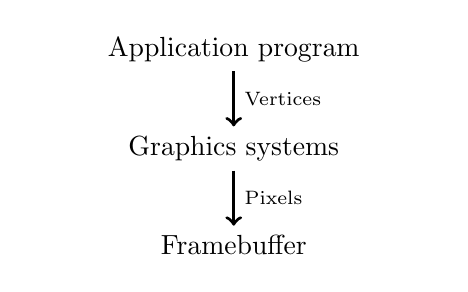
\begin{tikzpicture}[node distance=0.7cm]
\node (0) at (0,0) {\begin{minipage}{5cm}\centering Application program \end{minipage}};
\node (1) [below=of 0] {\begin{minipage}{5cm}\centering Graphics systems \end{minipage}};
\node (2) [below=of 1] {\begin{minipage}{5cm}\centering Framebuffer \end{minipage}};
\draw[->,very thick](0)to node[right] {\scriptsize{Vertices}}(1);
\draw[->,very thick](1)tonode[right] {\scriptsize{Pixels}}(2);
\end{tikzpicture}
\end{karte}

\begin{karte}[CGIS]{Weg der Daten zum Bildschirm (mit Grafik-Pipeline): Graphics systems}[Graph. Datenverarb.]
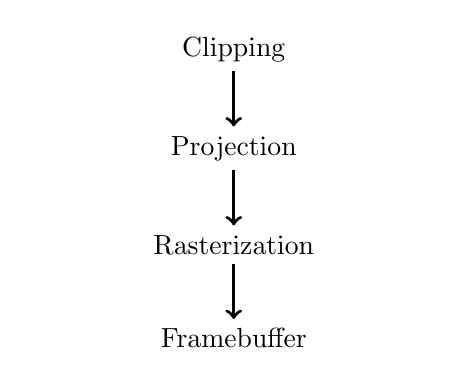
\begin{tikzpicture}[node distance=0.7cm]
\node (0) at (0,0) {\begin{minipage}{5cm}\centering Clipping \end{minipage}};
\node (1) [below=of 0] {\begin{minipage}{5cm}\centering Projection\end{minipage}};
\node (2) [below=of 1] {\begin{minipage}{5cm}\centering Rasterization \end{minipage}};
\node (3) [below=of 2] {\begin{minipage}{5cm}\centering Framebuffer \end{minipage}};
\draw[->,very thick](0)to (1);
\draw[->,very thick](1)to (2);
\draw[->,very thick](2)to (3);
\end{tikzpicture}
\end{karte}

\begin{karte}[CGIS]{Ablauf}[Fragmentbearbeitung]
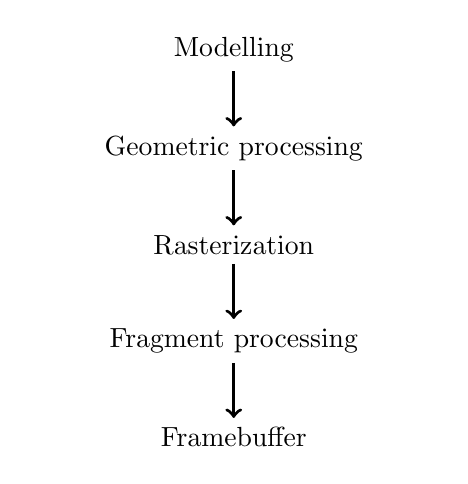
\begin{tikzpicture}[node distance=0.7cm]
\node (0) at (0,0) {\begin{minipage}{5cm}\centering Modelling \end{minipage}};
\node (1) [below=of 0] {\begin{minipage}{5cm}\centering Geometric processing\end{minipage}};
\node (2) [below=of 1] {\begin{minipage}{5cm}\centering Rasterization \end{minipage}};
\node (3) [below=of 2] {\begin{minipage}{5cm}\centering Fragment processing \end{minipage}};
\node (4) [below=of 3] {\begin{minipage}{5cm}\centering Framebuffer \end{minipage}};
\draw[->,very thick](0)to (1);
\draw[->,very thick](1)to (2);
\draw[->,very thick](2)to (3);
\draw[->,very thick](3)to (4);
\end{tikzpicture}
\end{karte}

\begin{karte}[CGIS]{4 Hauptaufgaben}[Fragmentbearbeitung]
\begin{itemize}
\item Modellierung (erzeugt Flächen und Vertices)
\item Geometrische Verarbeitung (arbeitet auf Flächen und Vertices)
\item Rasterisierung (erzeugt Fragmente)
\item Fragmentverarbeitung
\end{itemize}
\end{karte}

\begin{karte}[CGIS]{Definition}[Fragmente]
\begin{itemize}
\item Postion (x,y,z)
\item Normale, Tiefe, Farbe, Alphawert (Transparenz)
\item Standardisierte Verarbeitung
\end{itemize}
\end{karte}

\begin{karte}[CGIS]{Was ist Clipping? (mit Skizze)}[Clipping]
Abschneiden von nicht sichtbarer Geometrie (außerhalb des Sichtvolumens)
\end{karte}

\begin{karte}[CGIS]{Frustum}[Clipping]
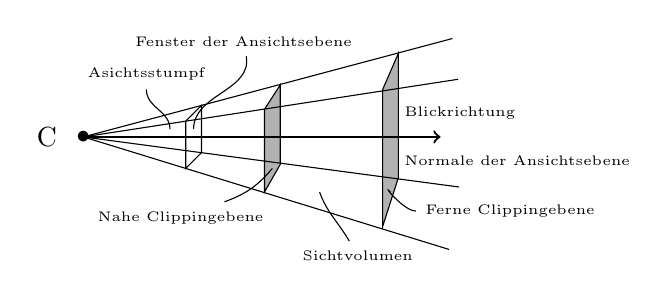
\begin{tikzpicture}[node distance=2cm]
\node[label={left:C}] (0) at (0,0) {$\bullet$};
\node[right=of 0,xshift=-1.1cm] (1) {};
\node[right=of 1] (2) {};
\node[right=of 2,xshift=-1.9cm,yshift=.3cm,label={right:\tiny{Blickrichtung}}](3){};
\node[right=of 2,xshift=-1.9cm,yshift=-.3cm,label={right:\tiny{Normale der Ansichtsebene}}](3){};
\node (ol1) at (1.3,.2) {};
\node (or1) at (1.5,.4) {};
\node (ul1) at (1.3,-.4) {};
\node (ur1) at (1.5,-.2) {};
\draw (ol1.center)--(or1.center)--(ur1.center)--(ul1.center)--(ol1.center);
\node (ol2) at (2.3,.35) {};
\node (or2) at (2.5,.66) {};
\node (ul2) at (2.3,-.7) {};
\node (ur2) at (2.5,-.35) {};
\draw [fill=black!30](ol2.center)--(or2.center)--(ur2.center)--(ul2.center)--(ol2.center);
\node (ol3) at (3.8,.6) {};
\node (or3) at (4,1.06) {};
\node (ul3) at (3.8,-1.14) {};
\node (ur3) at (4,-.52) {};
\draw [fill=black!30](ol3.center)--(or3.center)--(ur3.center)--(ul3.center)--(ol3.center);
\draw($(0)!-0mm!(ol1)$)--($(ol1)!-35mm!(0)$);
\draw($(0)!-0mm!(or1)$)--($(or1)!-33mm!(0)$);
\draw($(0)!-0mm!(ul1)$)--($(ul1)!-35mm!(0)$);
\draw($(0)!-0mm!(ur1)$)--($(ur1)!-33mm!(0)$);
\draw[->,thick]($(0)!-0mm!(1)$)--($(1)!-33mm!(0)$);
\node (fce) [below right=of 2, xshift=-.8cm, yshift=0.8cm] {\tiny{Ferne Clippingebene}};
\draw (fce)to[out=180](3.9,-.7);
\node (sv) [below =of 2, yshift=0.8cm] {\tiny{Sichtvolumen}};
\draw (sv)to[out=120,in=290](3,-.7);
\node (nce) [below=of 1, yshift=1.3cm] {\tiny{Nahe Clippingebene}};
\draw (nce)to[out=20,in=230](2.4,-.4);
\node (fae) [above=of 1,xshift=.8cm, yshift=-1.1cm] {\tiny{Fenster der Ansichtsebene}};
\draw (fae)to[out=280,in=90](1.4,.1);
\node (as) [above=of 0, xshift=.8cm, yshift=-1.6cm] {\tiny{Asichtsstumpf}};
\draw (as)to[out=270,in=90](1.1,.1);
\end{tikzpicture}
\end{karte}

\begin{karte}[CGIS]{Warum?}[Clipping]
\begin{itemize}
\item Entlastung der Rasterung
\item bessere Performance
\end{itemize}
\end{karte}

\begin{karte}[CGIS]{Was sind darzustellende Objekte?}[Clipping]
\begin{itemize}
\item vollständig im Sichtvolumen (kein Clipping)
\item vollständig außerhalb des Sichtvolumens (kein Clipping)
\item teilweise im Sichtvolumen (Clipping)
\end{itemize}
\end{karte}

\begin{karte}[CGIS]{Welche Arten gibt es und wann verwendet man sie?}[Clipping]
\begin{itemize}
\item geometrisch/analytisch bei der Geometrieverarbeitung $\rightarrow$ geometrische Objekte sind oft sehr groß (viele  Fragmente), daher lohnt geometrisches Clipping
\item Scissoring (nach dem Rastern im Framebuffer) $\rightarrow$ ausschließlich bei nur gerasterten Objekten, z.B. Schriften
\item Standardisierte Verarbeitung
\end{itemize}
\end{karte}

\begin{karte}[CGIS]{Problem beim Clipping von Polygonen}[Clipping]
konkave Polygone können "`zerfallen"', müssen vor der Verarbeitung tesseliert werden (in Dreiecke umgewandelt), da OpenGL nur konvexe Polygone unterstützt
\end{karte}

\begin{karte}[CGIS]{Was ist Culling}[Clipping]
Das Entfernen nicht benötigter Geometrie, die innerhalb des Sichtvolumens liegt.
\end{karte}

\begin{karte}[CGIS]{Welche Cullingarten gibt es?}[Clipping]
\begin{itemize}
\item Backface Culling: Entfernen von Primitiven "`mit dem Rücken zur Kamera"', verfügbar in OpenGL\\
bei geschlossenen Objekten: Flächen mit $N_p \cdot N > O$ werden beseitigt, wobei gilt: $N_p =$ Normale der Fläche, $N =$ Sichtlinie
\item Occlusion Culling: Entfernen von Geometrie, die von anderer überdeckt wird
\item Viewfrustum Culling: Entfernen von Geometrie, die außerhalb des Sichtvolumens liegt, vgl. Clipping
\end{itemize}
\end{karte}

\begin{karte}[CGIS]{Welche Probleme treten beim Culling auf?}[Clipping]
\begin{itemize}
\item keine Szeneninformationen vorhanden, aber für viele Cullingtechniken benötigt
\item geometrisch komplex
\end{itemize}
\end{karte}

\begin{karte}[CGIS]{Was ist Rasterung}[Rasterung]
\begin{itemize}
\item Abbildung eines analytisch beschriebenen Objektes auf ein diskretes Raster
\item Schritt von Geometrie zum Fragment
\item zentrales Element der Rendering-Pipeline
\item erfordert effizienten Algorithmus
\end{itemize}
\end{karte}

\begin{karte}[CGIS]{Rasterung von Kreisen für die FUnktion $F(x,y) = x^2 + y^2 - R^2$, wobei gilt: $R=$ Radius}[Rasterung]
Falls $F(x,y)$
\begin{itemize}
\item [$=0$] Punkt liegt auf dem Kreis
\item [$<0$] Punkt liegt innerhalb des Kreises
\item [$>0$] Punkt liegt außerhalb des Kreises
\end{itemize}
Liegt der Mittelpunkt zwischen E und SE außerhalb des Kreises, wähle SE; liegt der Mittelpunkt innerhalb des Kreises, wähle E.
\end{karte}

\begin{karte}[CGIS]{Rasterung von Polygonen}[Rasterung]
\begin{itemize}
\item Füllen entlang einer (horizontalen) Scanlinie
\item Wichtig: Innen-/Außentest für Pixel auf der Linie
\end{itemize}
\end{karte}

\begin{karte}[CGIS]{Scanline-Algorithmus}[Rasterung]
\begin{itemize}
\item zeilenweises "`scannen"' des Bildraumes
\item pro Scanline:
	\begin{itemize}
	\item Berechnung von Schnittpunkt mit gegebenem Primitiv
	\item Sortieren der Schnittpunkte
	\item Schnittpunktpaare nach "`Ungeradzahligkeitsregel"' bilden einen "`Span"'
	\item Verarbeiten der zu "`Spans"' gehörigen Pixel
	\end{itemize}
\item Ungeradzahligkeitsregel:
	\begin{itemize}
	\item Zeichnen von Pixel zwischen Paaren von SPs
	\item Pixel mit $s_{2n} < x < s_{2n +1}$ innerhalb des Polygons, Pixel mit $s_{2n+1} < x < s_{2n}$ außerhalb
	\end{itemize}
\end{itemize}
\end{karte}

\begin{karte}[CGIS]{Welche Algorithmen gibt es für das Sichtbarkeitsproblem?}[Sichtbarkeit]
\begin{itemize}
\item Objektraumalgorithmen: Berechnung in Weltkoordinaten des jeweiligen Modells\\
	 Vorteile: hohe Detailauflösung und Genauigkeit, analytische Ausgabe der Resultate\\
	 Nachteile: komplexe Verfahren, schwer parallelisierbar/implementierbar
\item Bildraumalgorithmen: Berechnung in Bildschirmkoordinaten\\
	 Vorteile: einfacher Verfahren, parallelisierbar/implementierbar
	Nachteile: beschränkte Genauigkeit, hohes Daten-/Speicherplatzaufkommen
\end{itemize}
\end{karte}

\begin{karte}[CGIS]{Welche Kategorien von Farbmodellen gibt es?}[Grafikprogrammierung]
\begin{itemize}
\item Technische (RGB,CMYK,YIQ)
\item Perzeptionsorientierte (HSV,HLS,Theoretische, CIE)
\end{itemize}
\end{karte}

\begin{karte}[CGIS]{additive Farbmischung}[Grafikprogrammierung]
Intensität wird addiert (Monitor, Projektor)\\
\ \\ RGB, CIE-Farbraum
\end{karte}

\begin{karte}[CGIS]{subtraktive Farbmischung}[Grafikprogrammierung]
Intensität wird subtrahiert (Drucker)\\
\ \\ CMYK
\end{karte}

\begin{karte}[CGIS]{wahrnehmungsorientierte Farbmischung}[Grafikprogrammierung]
Grundkomponenten: Sättigung, Helligkeit, Farbton/Farbe\\
\ \\ HSV
\end{karte}

\begin{karte}[CGIS]{Plenoptische Funktion}[Beleuchtung]
\begin{itemize}
\item 6-dimensionale Funktion
\item methematische Beschreibung dessen, was wir sehen
\item alle Strahlen an allen Punkten
\end{itemize}
\end{karte}

\begin{karte}[CGIS]{Lichtmodelle}[Beleuchtung]
\begin{itemize}
\item geometrische Optik: Emission, Reflektion/Refraktion, Absorbtion, wird in der CG verwendet
\item Wellenmodelle: Objektgröße vergleichbar mit Wellenlänge, Beugung, Interferenz, Polarisierung
\item Quantenmodelle: Fluoressenz, Phosphoressenz
\end{itemize}
\end{karte}

\begin{karte}[CGIS]{Was kann mit Licht passieren, wenn es auf eine Oberfläche trifft?}[Grafikprogrammierung]
\begin{itemize}
\item absorbiert
\item reflektiert
\item gestreut (in viele Richtungen reflektiert)
\item gebrochen
\item weitergeleitet
\end{itemize}
\end{karte}

\begin{karte}[CGIS]{Welche Vorraussetzungen hat die geometrische Optik?}[Beleuchtung]
\begin{itemize}
\item Licht breitet sich gradlinig aus
\item Strahlen interagieren nicht miteinander (Summation)
\item Strahlen haben Farbe (Wellenlänge) und Intensität
\end{itemize}
\end{karte}

\begin{karte}[CGIS]{Renderinggleichung - Theorie}[Beleuchtung]
\begin{itemize}
\item beschreibt den Energietransport in einer Szene
\item Eingabe:
	\begin{itemize}
	\item Lichtquellen
	\item Geometrie der Flächen
	\item Reflektionsverhalten (Material) der Flächen
	\end{itemize}
\item Ausgabe: Radianzwerte an Oberflächenpunkten für alle Richtungen
\end{itemize}
\end{karte}

\begin{karte}[CGIS]{Annahmen bei OpenGL}[Beleuchtung]
\begin{itemize}
\item Punktlichtquellen
\item nur direkte Beleuchtung
\item Materialien: diffus, glänzend oder transparent
\end{itemize}
\end{karte}

\begin{karte}[CGIS]{Was tut eine Beleuchtungsmethode?}[Beleuchtung]
\begin{itemize}
\item berechnet das reflektierende Licht an einem Ort auf einer Oberfläche
\item verwendet lokale oder globale Beleuchtungsmodelle
\item arbeitet in Weltkoordinaten
\end{itemize}
\end{karte}

\begin{karte}[CGIS]{Für was sind Schattierungsverfahren?}[Shading]
\begin{itemize}
\item bestimmt die Reflektion aller Pixel eines Polygons
\item Voraussetzung: Beleuchtungsmethode für die Bestimmung einzelner Pixelweerte vorhanden
\item arbeitet in Bildschirmkoordinaten
\end{itemize}
\end{karte}

\begin{karte}[CGIS]{Shadingarten}[Shading]
\begin{itemize}
\item Flatshading: nur 1 Helligkeitswert/Polygon \\(Beobachter im Unendlichen), einmalige Auswertung der Beleuchtungsgleichung
\item Gourandshading: \scriptsize{"Normalen" in Eckpunkten bestimmen, hieraus wird die Intensität berechnet, Werte aus dieser Berechnung werden zur Berechnung der Drei- und Vierecke herangezogen $\rightarrow$ Intensitäten werden für Helligkeitsbestimmung interpoliert}
\item \normalsize Phongshading: Normalen aus den Normalen in den Eckpunkten werden interpoliert, diese werden dann zur Helligkeitsberechnung/Pixel verwendet
\end{itemize}
\end{karte}

\begin{karte}[CGIS]{Pixel-Pipeline}[OpenGL]
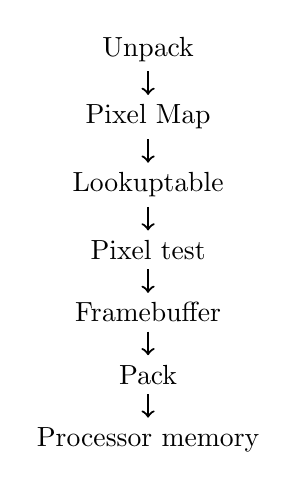
\begin{tikzpicture}[node distance=0.3cm]
\node (0) at (0,0) {Unpack};
\node (1) [below=of 0] {Pixel Map};
\node (2) [below=of 1] {Lookuptable};
\node (3) [below=of 2] {Pixel test};
\node (4) [below=of 3] {Framebuffer};
\node (5) [below=of 4] {Pack};
\node (6) [below=of 5] {Processor memory};
\draw[->,thick] (0)to (1);
\draw[->,thick] (2)to (3);
\draw[->,thick] (4)to (5);
\draw[->,thick] (1)to (2);
\draw[->,thick] (3)to (4);
\draw[->,thick] (5)to (6);
\end{tikzpicture}
\end{karte}

\begin{karte}[CGIS]{Pixel und Geometrie-Pipeline}
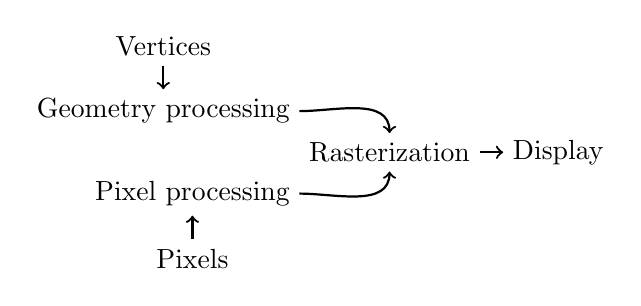
\begin{tikzpicture}[node distance=0cm]
\node (0) at (0,0) {Vertices};
\node (1) [below=of 0,yshift=-0.3cm] {Geometry processing};
\node (2) [below right=of 1] {Rasterization};
\node (3) [below left=of 2] {Pixel processing};
\node (4) [below=of 3,yshift=-.3cm] {Pixels};
\node (5) [right=of 2,xshift=.3cm] {Display};
\draw[->,thick] (0)to [out=270,in=90](1);
\draw[->,thick] (1)to [out=0,in=90](2);
\draw[->,thick] (3)to [out=0,in=270](2);
\draw[->,thick] (4)to [out=90,in=270](3);
\draw[->,thick] (2)to [out=0,in=180](5);
\end{tikzpicture}
\end{karte}



\end{document}